%
% filter.tex -- Paper zum Thema Optische Fouriertransformation <opt>
%
% (c) 2023 Marco Niederberger, Yanick Schoch; OST Ostschweizer Fachhochschule
%
% !TEX root = ../../buch.tex
% !TEX encoding = UTF-8
%
\section{Filter
\label{opt:section:filter}}
\rhead{Filterdesign}

Auch bei der optischen Fouriertransformation kann das Signal anschliessend in der Fourierebene bearbeitet werden.
Im optischen entspricht dies einer Blende.
Diese wird, wie in Abbildung \ref{opt:fig:4fAufbau} gezeigt, zwischen den beiden Linsen platziert.
Typische Filter in der Elektrotechnik sind Tiefpass, Hochpass, Bandpass und Bandsperre.
Deren Realisierung in der Optik ist in Abbildung \ref{opt:fig:filterarten} ersichtlich.

Im Nullpunkt der Filterebene sind die tiefen Frequenzen (DC-Anteil) und entlang der Achsen die höheren Frequenzen zu erkennen.
Somit entspricht eine lichtundurchlässige Fläche mit einem Loch in der Mitte einem Tiefpass und eine lichtundurchlässige Scheibe einem Hochpass.
Nach diesem Prinzip lassen sich auch die weiteren typischen Filter realisieren.

\begin{figure}
    \centering
    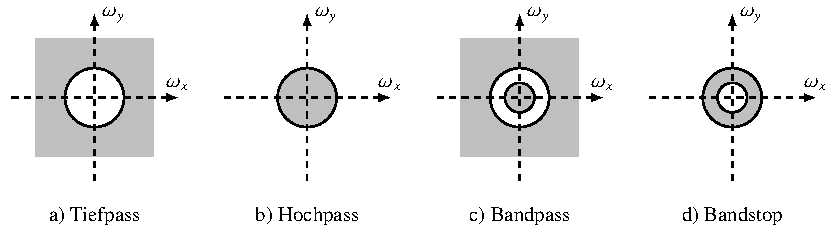
\includegraphics[width=\textwidth]{papers/opt/images/filterarten.pdf}

    \caption{Realisierung typischer Filter als optische Systeme;
        wobei grau lichtundurchlässig und weiss lichtdurchlässig bedeutet.}
    \label{opt:fig:filterarten}
\end{figure}

\subsection{Anwendung in der Bildverarbeitung}
\label{opt:section:image_processing}

Wie in Kapitel \ref{opt:section:filter} gezeigt kann in der Fourierebene gefiltert werden.
Im folgenden wird dies an einem Bild und mehreren Filtern illustriert.
In Abbildung \ref{opt:fig:image_raw} ist das Originalbild sowie dessen Fouriertransformation zu sehen.
Dabei entspricht die Farbe weiss im Spektrum einer hohen Energie und die Farbe schwarz einer tiefen Energie.

Das besagte Spektrum wird in Abbildung \ref{opt:fig:image_lowpass} mit einem Tiefpass gefiltert.
Wie bereits erwähnt entspricht ein Tiefpass im Optischen einer Blende, welche alles Licht ausserhalb eines Kreises blockiert.
Das so entstehende Spektrum wird rücktransformiert und führt zu einer unscharfen Kopie des Originalbildes.

Abbildung \ref{opt:fig:image_highpass} zeigt genau das Gegenteil. 
Das Spektrum wird mittels Hochpass gefiltert, das bedeutet, dass eine Kreisfläche geblockt und alles andere durchgelassen wird.
Die Rücktransformation dieser Filterung betont die scharfen Kanten des Originalbildes. 

\begin{figure}
    \centering
    \subfigure{
        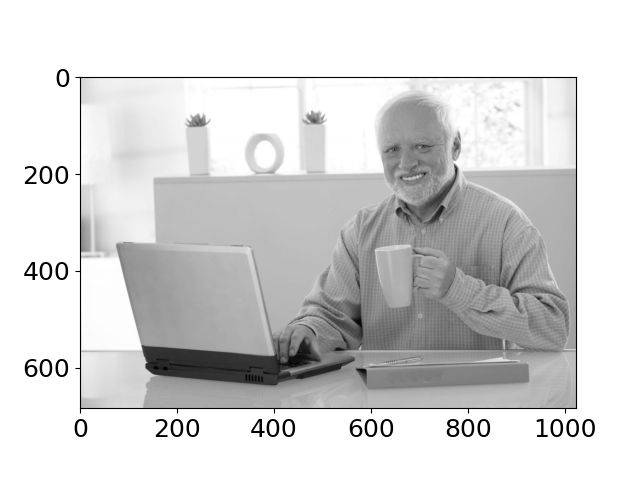
\includegraphics[width=0.4\textwidth]{papers/opt/images/harold.png}
    }
    \subfigure{
        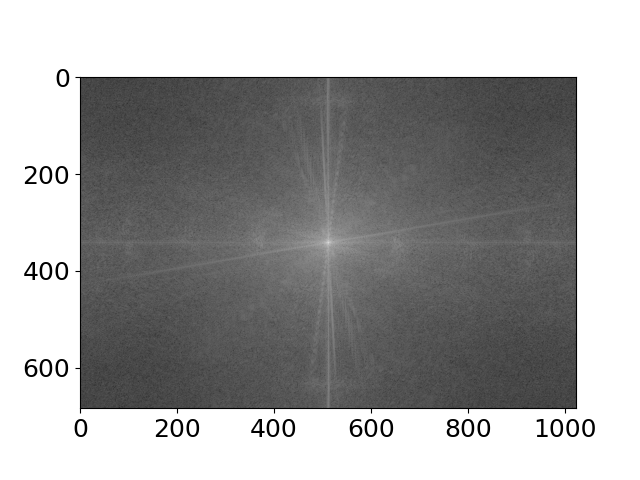
\includegraphics[width=0.4\textwidth]{papers/opt/images/harold_fourier.png}
    }

    \caption{Beispielbild und dessen Fouriertransformation.
    Im Zentrum sind die tiefen und am Rande die hohen Frequenzen ersichtlich.
    Dabei entspricht die Farbe weiss im Spektrum einer hohen Energie und die Farbe schwarz einer tiefen Energie.}
    \label{opt:fig:image_raw}
\end{figure}

\begin{figure}
    \centering
    \subfigure{
        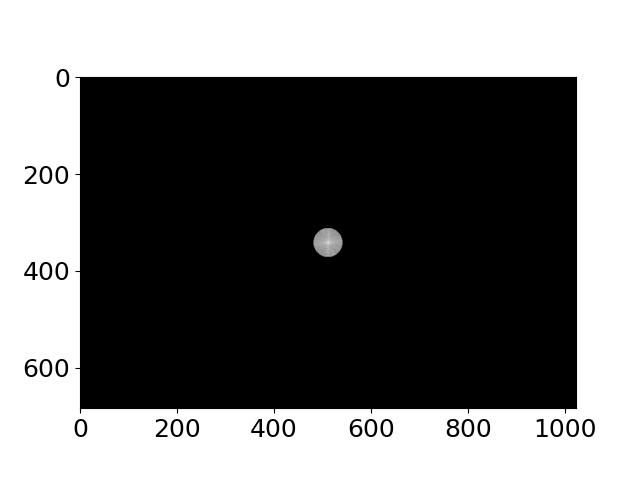
\includegraphics[width=0.4\textwidth]{papers/opt/images/harold_fourier_lowpass.png}
    }
    \subfigure{
        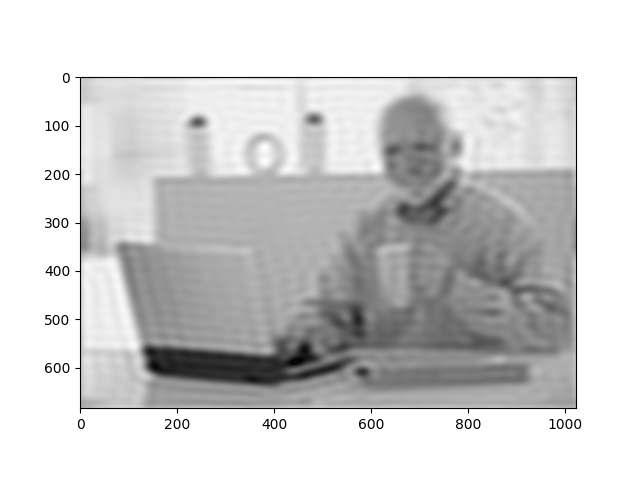
\includegraphics[width=0.4\textwidth]{papers/opt/images/harold_reconstructed_lowpass.png}
    }

    \caption{Das Spektrum aus Abbildung \ref{opt:fig:image_raw} wird mit einem Tiefpass gefiltert und wieder rücktransformiert.
    Das rücktransformierte Bild ergibt eine verwaschene Kopie des Originalbildes.}
    \label{opt:fig:image_lowpass}
\end{figure}

\begin{figure}
    \centering
    \subfigure{
        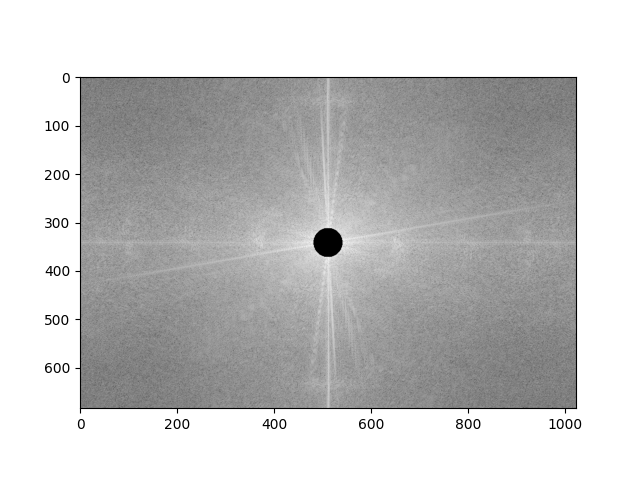
\includegraphics[width=0.4\textwidth]{papers/opt/images/harold_fourier_highpass.png}
    }
    \subfigure{
        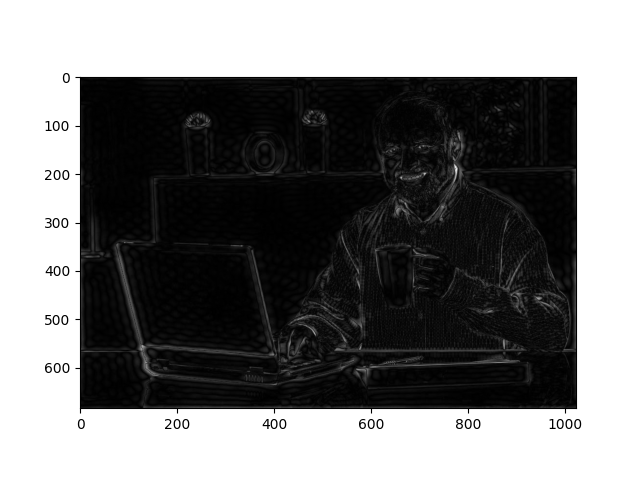
\includegraphics[width=0.4\textwidth]{papers/opt/images/harold_reconstructed_highpass.png}
    }

    \caption{Das Spektrum aus Abbildung \ref{opt:fig:image_raw} wird mit einem Hochpass gefiltert und wieder rücktransformiert.
    Das rücktransformierte Bild betont die harten Kanten im Originalbild.}
    \label{opt:fig:image_highpass}
\end{figure}
